\documentclass[11pt]{beamer}
\usepackage[utf8]{inputenc}
\usepackage[spanish]{babel}
\usepackage{amsmath}
\usepackage{amsfonts}
\usepackage{amssymb}
\usepackage{graphicx}
\usepackage{caption}
\usepackage{subcaption}
\usepackage{lipsum}
\usepackage{ragged2e}
\usepackage{hyperref}
\usepackage{float}
\usepackage{url}
\usepackage{multicol}
\usetheme{Madrid}
\newcommand{\celda}[1]{
	\begin{minipage}{2.5cm}
		\vspace{5mm}
		#1
		\vspace{5mm}
	\end{minipage}
}
\newtheorem{teorema}{Teorema}[section]
\newtheorem{proposicion}{Proposición}[section]
\newtheorem{definicion}{Definición}[section]
\newtheorem{nota}{Nota}[section]
\newtheorem{corolario}{Corolario}[section]

\author[Christian Paredes A.]{\footnotesize Christian Paredes Aguilera \\ \vspace{4mm} En colaboración con:\\ \vspace{1mm} Gabriel Rosario Roselló  \\ Jorge Valero \\\vspace{4mm} {\color{blue} XI Congreso InvestMat}}
\title [XI Congreso InvestMat] {Coherencia wavelet, una herramienta para el análisis dinámico entre series temporales.}
\date{10 Enero 2024} 

\logo{
    
\includegraphics[width=1cm,height=1cm,keepaspectratio]{logouv.jpg}
    
\includegraphics[width=1cm,height=1cm,keepaspectratio]{upvlogo.jpg}
    }



%\AtBeginSection[]
%{
%	\begin{frame}<beamer>{Índice}
%		\tableofcontents[currentsection,currentsubsection]
%	\end{frame}
%}


\begin{document}
\begin{frame}
		\maketitle
	\end{frame}

	\begin{frame}{\footnotesize Coherencia wavelet, una herramienta para el análisis dinámico entre series temporales.}
		\tableofcontents
	\end{frame}
	
\section{Introducción}
	

    % ------------------------ INTRODUCCIÓN ------------------------
    \begin{frame}{Introducción}

	Existen diversas técnicas, para analizar completamente dos variables a lo largo del tiempo:
	\vspace{5mm}
	\begin{itemize}
	    \item Coeficiente de correlación de Pearson $\rightarrow$ \textbf{Correlación}.
	    \item Series de Fourier $\rightarrow$ \textbf{Frecuencia}.
	    \item Causalidad de Granger $\rightarrow$ \textbf{Causalidad}.
	\end{itemize}
    \end{frame}

    %PÁGINA 4
    \begin{frame}{Introducción}

	\begin{center}
	    ¿Existe otra técnica que sea capaz de análisis conjuntamente la Correlación, la Frecuencia, la Causalidad y más?
	\end{center}

	\begin{center}
	    SI!!!
	\end{center}

	\begin{center}
	    WAVELETS: Coherencia wavelet y diferencia de fase.
	\end{center}

    \end{frame}

    %PÁGINA 5
    \begin{frame}{Introducción}{Ventajas de usar wavelets}
	Ventajas de usar wavelets en series de tiempo:
	\vspace{5mm}
	\begin{itemize}	
	    \item Resolución en tiempo y frecuencia.
	    \item Análisis multiescala.
	    \item Manejo de datos no estacionarios.
	\end{itemize}

    \end{frame}

    %PÁGINA 6
    \begin{frame}{Introducción}{Definición de coherencia wavelet}
	Cuando hablamos de coherencia wavelet, nos referimos a una relación dinámica.

	\begin{definicion}
	    La coherencia wavelet entre dos series de tiempo $x(t)$ e $y(t)$ es una función de tiempo y escala definida por:
	    \begin{equation}
		R^{2}_{xy}(\tau,s)=\frac{\left|S\left(s^{-1}W_{xy;\psi(\tau,s)}\right)\right|^2}{S\left(s^{-1}\left|W_{x;\psi}(\tau,s)\right|^2\right)S\left(s^{-1}\left|W_{y;\psi}(\tau,s)\right|^2\right)}
	    \end{equation}
	\end{definicion}

    \end{frame}

    %PAGINA 7
    \begin{frame}{Introducción}{Ejemplo}
	Demos un ejemplo:

	\begin{center}
	    Café vs. $\pi$zzas
	\end{center}
	%2 columnas 
	\begin{multicols}{2}
	     \begin{figure}
		 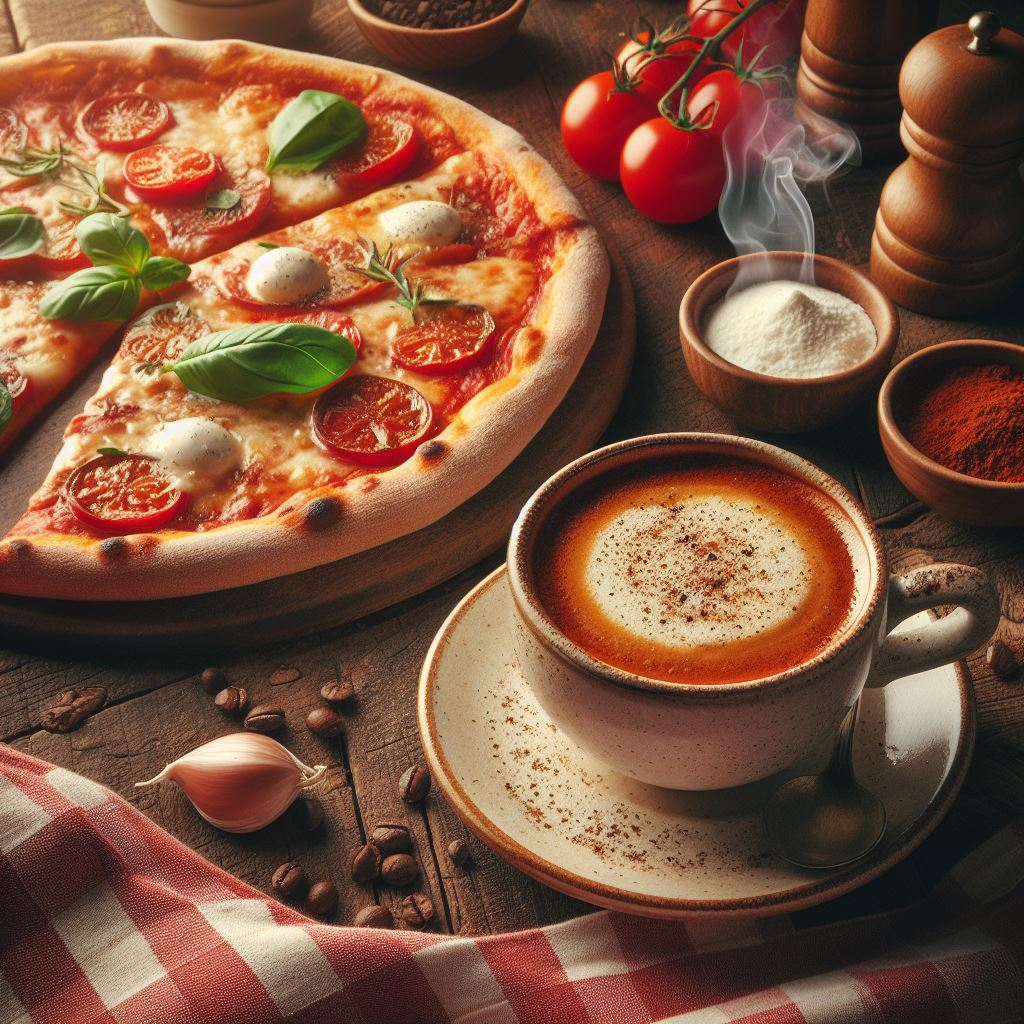
\includegraphics[scale=0.12]{cafePizza.jpeg}
		 %\caption{Morlet Wavelet $\psi=e^{-t^2/2}cos(5t)$}
		 %\label{fig:enter-label}
	     \end{figure}
	     $\frac{\left|S\left(s^{-1}W_{xy;\psi(\tau,s)}\right)\right|^2}{S\left(s^{-1}\left|W_{x;\psi}(\tau,s)\right|^2\right)S\left(s^{-1}\left|W_{y;\psi}(\tau,s)\right|^2\right)}$
	     \vspace{5mm}
	    En pocas palabras la coherencia wavelet es el grado con el que \textbf{correlacionan} dos series de temporales en función del \textbf{tiempo} y la \textbf{frecuencia}.
	\end{multicols}

    \end{frame}

	
    %PAGINA 8
    % ------------------------ OBJETIVO ------------------------
    \begin{frame}{Objetivo}

	Ahora, para hablar de \textbf{causalidad}, necesitamos definir \textbf{diferencia de fase}. Que será el objetivo de esta presentación, seguido de detallar los \textbf{datos} analizados y presentar \textbf{resultados} empíricos.

    \end{frame}


\section{Construcción}
    \subsection{Definición de diferencia de fase}
    
	%PAGINA 10
	\begin{frame}
	    \begin{definicion}

	    \end{definicion}
	 \end{frame}



    \section{Conlusión}
    \begin{frame}{Conclusión}
        Así pues, como ya conocemos la \textbf{correlación}, sabemos que esta relación nos da un indicadador, en este caso, entre la distribución de las potencias entre dos series temporales a cada tiempo.
        
        \vspace{3mm}
        Este indicador pero, tiene un inconveniente, ya que esta definido como un cuadrado, y {\color{red} no podemos distinguir entre correlacion positiva y negativa}.

        \vspace{3mm}
        \begin{center}
        {\large \textbf{¿Cómo podemos solucionarlo?}}
        \end{center}
    \end{frame}

    \begin{frame}{Fin}
    \begin{center}
        {\huge Fin}
        
        \vspace{5mm}
        {\large ¡Muchas gracias por vuestra atención!}
    \end{center}
    \end{frame}

    \section{Bibliografía}
    \begin{frame}{Bibliografía}
        \begin{thebibliography}{99}


    \bibitem{POR} 
    \textsc{Aguiar-Conraria, L., Azevedo, N. \& Soares, M.J.}, \textit{Using wavelets to decompose the time-frequency effects of monetary policy}, Physica A: Statistical Mechanics and its Applications {\bf 387}  (2008), pp., 2863-2878.  
    
    \bibitem{MGI2015} 
    \textsc{Jiang, C., Chang, T., Li XL.}, \textit{Money growth and inflation in China: New evidence from a wavelet analysis}, International Review of Economics \& Finance {\bf 35}, (2015), pp. 249-261. 

    \bibitem{PGWA} 
    \textsc{Torrence C. \& Compo, G.}, \textit{A Practical Guide to wavelet analysis}, Bulletin of the American Meteorological Society {\bf 79}  (1998), pp., 61-78.  

    \bibitem{BCE}
    \href{https://data.ecb.europa.eu/data}{European Central Bank}

\end{thebibliography}
    \end{frame}
	
\end{document}
